\documentclass[../main.tex]{subfiles}
\begin{document}
\chapter{FedRAMP - Federal Risk and Authorization Management Program}
\section{Introduzione}
In questo capitolo verrà approfondito FedRAMP, il programma federale americano per la gestione del rischio e delle autorizzazioni nella cloud.
Sarà proposta un'analisi degli obiettivi del programma, specificando le problematiche in esso affrontate in relazione anche a quanto descritto nel capitolo precedente.
Verrà poi esposta la struttura del documento, dopodiché ci si concentrerà sulla struttura dello stesso approfondendo i ruoli degli attori coinvolti, e il contributo che questo lavoro di tesi vuole apportare per ciascun caso trattato.
In conclusione saranno esposti i concetti di \textit{readiness} e di \textit{compliance} al programma, e sarà approfondita l'implementazione di FedRAMP in Amazon AWS.

\section{Cos'è FedRAMP}
FedRAMP è il programma governativo americano l'applicazione del \textbf{FISMA} (Federal Information Security Management Act) nell'adozione di tecnologie cloud.
Esso propone un approccio standardizzato al \textit{security assessment}, alle autorizzazioni e al monitoraggio continuo di prodotti e servizi cloud, fornendo un insieme di requisiti di sicurezza e un programma di assessment indipendente, nato dalla collaborazione di esperti di sicurezza e di tecnologie cloud.
Le entità coinvolte nella redazione di questo programma sono state molte: la General Services Administration (GSA), il National Institute of Standards and Technology (NIST), il dipartimento di Sicurezza Nazionale (Department of Homeland Security, DHS), il dipartimento della Difesa (Department of Defense, DOD), la National Security Agency (NSA), l'Office of Management and Budget (OMB).

I \textit{cloud service provider} che vogliono offrire servizi per la pubblica amministrazione americana e gli uffici federali devono essere autorizzati tramite questo programma.
Nonostante sia stato sviluppato nel contesto USA, la dinamicità e l'elasticità di FedRAMP ne ha permesso l'adozione \textit{de-facto} anche in altre nazioni, specialmente dell'Asia orientale e del nord Europa.
\subsection{FISMA, Federal Information Security Management Act}
Il FISMA è uno standard di sicurezza, entrato in vigore come legge il 17 Dicembre 2002 come "Titolo III" dell'E-Government Act\cite{united2004information}: ciascun sistema che ospiti dati governativi deve essere autorizzato tramite il FISMA prima di essere messo in produzione.
Esso definisce tre obiettivi principali per la sicurezza dei sistemi informativi federali:
\begin{itemize}
    \item \textbf{Confidenzialità}, per garantire restrizioni autorizzate sull'accesso e la \textit{disclosure} dei dati, con l'obiettivo di proteggere la privacy ed eventuale informazioni sul proprietario odegli stessi
    \item \textbf{Integrità}, per proteggere il dato da manipolazioni o azioni distruttive e per garantire allo stesso tempo l'autenticità e la non-repudiabilità dell'informazione
    \item \textbf{Disponibilità}, per assicurare condizioni di affidabilità nell'accesso al dato
\end{itemize}

A tal fine il \textbf{NIST} ha prodotto il \textbf{Federal Information Risk Management Framework}(\textit{RMF}) il quale organizza i sistemi informatici sulla base del livello di rischio e descrive un insieme minimo di requisiti che devono essere rispettati per garantire un livello di sicurezza adeguato\cite{nist2003nist}, fornendo una metodologia per la selezione dei controlli di sicurezza e per l'esecuzione del deployment e dell'assessment.

\begin{figure}[H]
\centering
\makebox[\textwidth]{
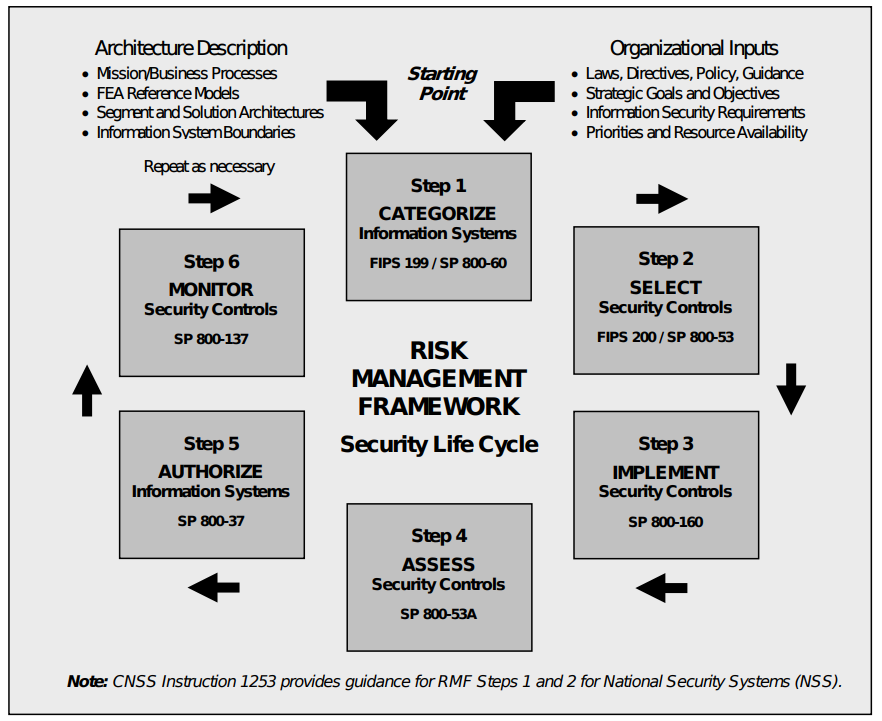
\includegraphics[width=0.8\textwidth]{immagini/risk_management_framework.png}
}
\caption{Risk Management Framework \cite{nist2003nist} }\label{fig:riskmanagementfw}
\end{figure}

Tramite la figura \ref{fig:riskmanagementfw} è possibile identificare le sei fasi che compongono il processo di gestione del rischio, ciclico e continuo, identificato dal framework:

\begin{itemize}
    \item \textbf{Categorizzazione del sistema informativo}, tramite i documenti FIPS\footnote{Federal Information Processing Standards} 199 e NIST SP 800-60 v2\cite{nist80060}. Il documento FIPS 199 classifica i sistemi in base al livello di rischio, e contiene i criteri da utilizzare nella categorizzazione. Questi criteri sono basati sull'impatto potenziale di una violazione delle proprietà di confidenzialità, integrità e disponibilità sul sistema e sono: i) Rischio basso, impatto limitato, ii) Rischio medio, con serie conseguenze, iii) Rischio elevato con conseguenze gravi e catrastofiche. FIPS 199 si applica a tutti i sistemi, ad esclusione di quelli designati per l'uso della sicurezza nazionale.
    \item \textbf{Selezione dei controlli di sicurezza}, mediante i documenti FIPS 200 e SP 800-53. FIPS 200 fornisce i requisiti di sicurezza minimi (e i relativi controlli) per ogni categoria definita nel FIPS 199.
        Il documento NIST 800-53\cite{nist2003nist} invece definisce i controlli di sicurezza e fornisce le linee guida per scegliere i profili da impiegare per soddisfare i requisiti minimi di sicurezza, in base all'impatto del sistema. I controlli di sicurezza sono divisi in 17 famiglie e vengono divisi in tre classi (controlli di gestione, controlli operazionali e controlli tecnici). 
    \item \textbf{Implementazione dei controlli}, guidata dal documento SP 800-160\cite{nist800160}
    \item \textbf{Assessment dei controlli di sicurezza}, regolato dal documento SP 800-53\cite{nist2003nist}
    \item \textbf{Autorizzazione del sistema informativo}, basata sul documento SP 800-37\cite{nist80037}
    \item \textbf{Fase di monitoraggio}\cite{nist800137}        
\end{itemize}

\subsection{Obiettivo di FedRAMP}
L'obiettivo di FedRAMP è quello di fornire un framework per semplificare il processo di autorizzazione dei servizi cloud adottati dagli enti governativi USA.
Prima dell'adozione di questo programma i produttori di sistemi e applicativi dovevano eseguire l'intero processo di autorizzazione per ciascuna delle agenzie che adottasse il sistema, così come ogni ente gestiva un processo di gestione del rischio a sé stante, anche nel caso in cui un'altra agenzia avesse già adottato servizi e misure di sicurezza analoghi. 
FedRAMP affronta la problematica nei seguenti modi\cite{understandingFedRAMP}:

\begin{itemize}
    \item Fornendo processi di valutazione della sicurezza e autorizzazione congiunti, basati su una serie di requisiti e controlli standardizzati, sulla base dell'impatto del sistema 
    \item Offrendo un programma di analisi della conformità in grado di produrre
    \item Strutturando un processo di analisi e valutazione della conformità condotto da Organizzazioni di terze parti approvate (3PAO), per valutare costantemente la capacità di un provider di servizi cloud (CSP) di soddisfare requisiti di sicurezza desiderati
    \item Coordinando servizi di monitoraggio continuo
    \item Fornendo pacchetti di autorizzazione composti da servizi cloud già revisionati da una Joint Authorization Board (JAB), composta da esperti di sicurezza provienienti dal DHS, dalla GSA e del DoD. 
    \item Offrendo un linguaggio standardizzato per aiutare i dipartimenti e gli enti governativi ad integrare i requisiti di FedRAMP all'interno dei processi interni
    \item Un repository di pacchetti di autorizzazione per i servizi cloud che possono essere utilizzati dal governo
\end{itemize}

L'utilizzo di un framework centralizzato ha inevitabilmente determinato un risparmio notevole anche in termini economici, sia per il governo americano, che per i cloud service provider: si stima che questo ammonti a circa \$250,000 per ciascun sistema autorizzato, per un totale di circa 160 implementazioni dello standard FISMA. Il risparmio stimato per il governo è quindi di 40 milioni di dollari \cite{7036263}.
\section{Struttura}
Il programma fornisce un percorso che i fornitori di servizi cloud possono intraprendere per ottenere una autorizzazione provvisoria, da sottoporre in una successiva fase di \textit{security assessment} che verrà poi revisionata dalla \textit{JAB}.
Mediante questo approccio preventivo è possibile quindi anticipare l'\textit{assessment} dei controlli di sicurezza e di velocizzare il processo di autorizzazione definitiva dell'applicativo o sistema cloud.
\subsection{CSP: FedRAMP readiness}

Il provider che vuole partecipare a FedRAMP deve innanzitutto soddisfare una serie di requisiti di \textit{readiness}:
\begin{enumerate}
    \item Essere in grado di trattare eventuali processi forensi elettronici e contenziosi 
    \item Essere in grado di definire e descrivere chiaramente i confini del proprio sistema
    \item Identificare le responsabilità del cliente e le azioni che questo deve compiere per implementare i controlli di sicurezza
    \item Fornire un meccanismo di identificazione e autenticazione a due fattori per l'accesso via rete agli account privilegiati
    \item Fornire un meccanismo di identificazione e autenticazione a due fattori per l'accesso via rete agli account non privilegiati
    \item Fornire un meccanismo di identificazione e autenticazione a due fattori per l'accesso locale agli account privilegiati
    \item Avere la possibilità di eseguire analisi del codice per le soluzioni software proprietarie
    \item Avere protezioni di confine garantendo isolamento logico e fisico degli asset
    \item Avere l'abilità di rimediare a situazioni di rischio elevato entro i 30 giorni (90 giorni per le situazioni di rischio moderato)
    \item Fornire un inventario e configurazioni standard per tutti i dispositivi
    \item Avere meccanismi di sicurezza che impediscano la fuoriuscita di informazioni nell'utilizzo di mezzi di comunicazione condivisi
    \item Adottare meccanismi di crittografia per preservare la confidenzialità e l'integrità dei dati trasmessi sulla rete
\end{enumerate}


Se queste condizioni sono rispettate, è possibile sottomettere un modulo di richiesta di ammissione al programma, disponibile online sul sito web di FedRAMP. A questo seguirà una notifica automatica all'ufficio di gestione del programma e alla \textit{Joint Advisory Board}.


Oltre alle finalità precedentemente esposte, il prodotto sviluppato in questo lavoro di tesi punta a supportare il processo di verifica dei requisiti richiesti per la \textit{readiness}. Poiché questi sono essenzialmente di carattere procedurale, saranno implementati sotto forma di questionario.
Per i punti 11 e 12 possono essere forniti anche controlli tecnici, legati però alle tecnologie effettivamente implementate.
%aggiungere eccdf

\subsection {Processo di autorizzazione}
\begin{figure}[H]
\centering
\makebox[\textwidth]{
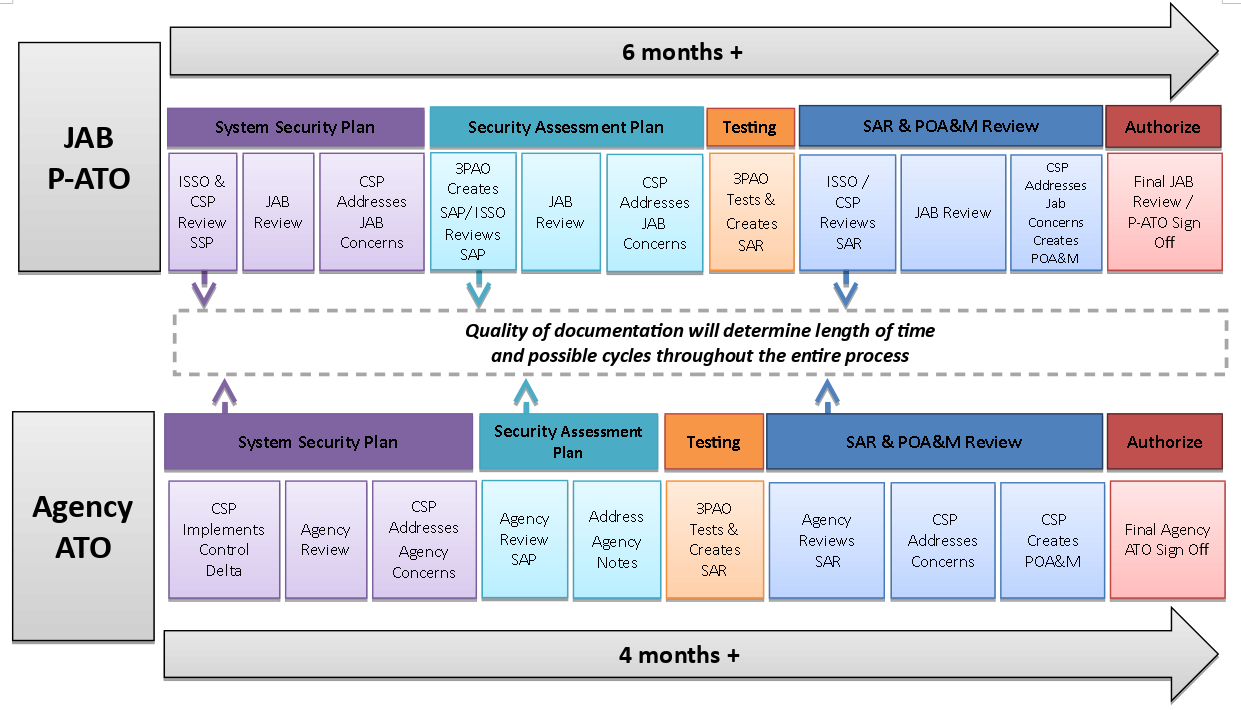
\includegraphics[width=\textwidth]{immagini/fedramp_process.png}
}
\caption{Processo di autorizzazione \cite{understandingFedRAMP} }\label{fig:fedramp_others}
\end{figure}


Nel modulo di richiesta di ammissione al programma il provider fornisce informazioni sul proprio sistema, categorizzandolo sulla base delle direttive contenute nel documento NIST SP 800-60 V2\cite{nist80060}, e decide la \textit{baseline} dei controlli di sicurezza da implementare in base alla sensibilità del sistema (bassa o media).
A seguito di una revisione della \textit{readiness} da parte dell'ufficio di gestione del programma, sarà possibile avviare il processo di richiesta dell'autorizzazione provisoria (P-ATO): il \textit{cloud service provider} deve quindi ricercare ed assumere un'organizzazione di terze parti, tra quelle specificate sul sito di FedRAMP.
L'attore principale è il fornitore di servizi, il quale sottometterà un \textit{security package} e sarà designato come candidato all'autorizzazione. Lo svolgimento del processo può avvenire in due modi:
\begin{itemize}
    \item \textit{Processo condotto da un'agenzia federale}, che vuole far autorizzare a FedRAMP i sistemi cloud correntemente attivi. In tal caso il processo è totalmente controllato e monitorato dall'ente, il cui compito è quello di sorvegliare sull'implementazione dei controlli di sicurezza mancanti nei sistemi del fornitore di servizi. L'autorizzazione sarà quindi emessa direttamente dall'agenzia.
    \item \textit{Processo mantenuto dalla Joint Authorization Board}, che analizzerà il livello di sicurezza del fornitore ed emetterà una autorizzazione provvisoria
\end{itemize}

\vfill
\subsubsection{Attori coinvolti nel processo di autorizzazione}
Gli attori coinvolti sono quindi gli enti federali che desiderano adottare un servizio cloud, i fornitori del servizio, e le organizzazioni di terze parti che ne effettuano l'analisi della sicurezza.

\begin{figure}[H]
\centering
\makebox[\textwidth]{
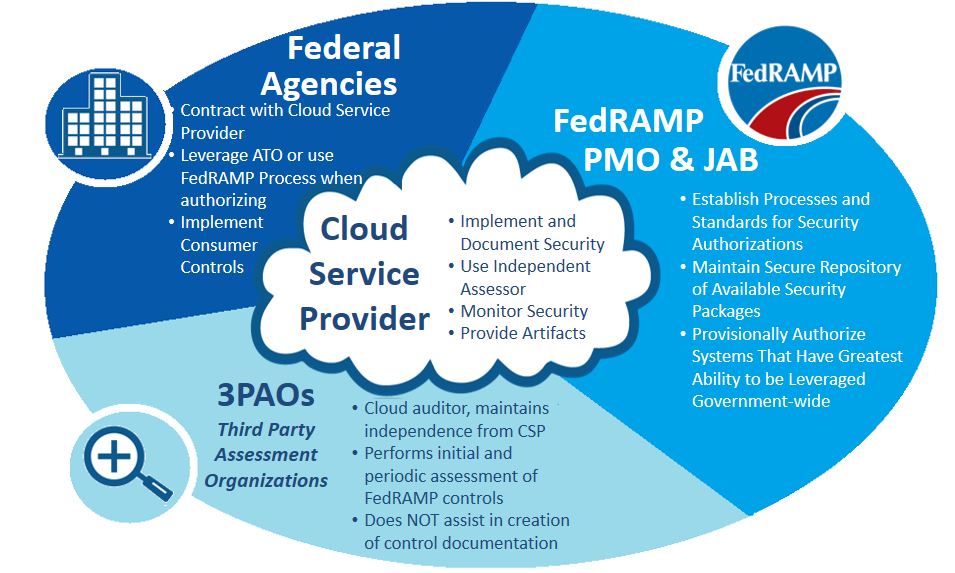
\includegraphics[width=\textwidth]{immagini/fedramp_actors.png}
}
\caption{Attori coinvolti nel processo di autorizzazione \cite{understandingFedRAMP} }\label{fig:fedrampactors}
\end{figure}



\subsubsection{Enti federali}
Il ruolo degli enti federali è quello di garantire che, per tutti i progetti nei quali sono coinvolte tecnologie cloud, siano rispettati i requisiti FedRAMP, venga effettuato l'assessment dei controlli di base, e siano stati forniti i template corretti.


Le agenzie devono catalogare i propri sistemi in un inventario, specificando quali di questi siano di tipo cloud e quali invece siano sistemi tradizionali. È raccomandabile avere un referente che sia preparato a rispondere a quesiti riguardanti l'implementazione dei requisiti FedRAMP.
Per facilitare ciò alcune informazioni utili potrebbero essere \textit{i) il nome del sistema cloud, ii) la descrizione del servizio fornito dal sistema, iii) il contatto dl proprietario del sistema, iv) la data di autorizzazione, v) lo stato della compliance}\cite{fedrampFramework}.


In fase di migrazione di sistemi tradizionali sul cloud, così come nell'adattamento di servizi cloud pre-esistenti a FedRAMP, è necessario che i requisiti del programma siano rispettati. Le agenzie devono quindi effetturare un'analisi approfondita delle conseguenze del cambio di tecnologia, per determinare i controlli di sicurezza aggiuntivi da effettuare.
Analogamente, gli stessi controlli di sicurezza devono interessare eventuali sistemi cloud installati ed utilizzati internamente (private-cloud). In tal caso è necessario predisporre un'analisi condotta da terze parti accreditate.
Se, invece, il fornitore del servizio è un privato e questi non ha effettuato l'assessment dei controlli di sicurezza FedRAMP, l'ente governativo è tenuto ad informare il provider e richiederne l'adeguamento immediato. 

Le agenzie, sulla base di specifiche esigenze, possono sottomettere eventuali controlli aggiuntivi rispetto a quelli basilari; questi devono devono essere adeguatamente documentati e motivati. Gli altri enti possono poi decidere di adottare questi controlli.
Allo stesso modo, come già trattato, le agenzie possono riutilizzare autorizzazioni emesse per altri enti.

Sulla base del E-Government Act del 2002 (Titolo III, Sezione 3544), le agenzie devono inoltre effettuare analisi del rischio periodiche, valutando l'impatto di eventuali violazione della confidenzialitàe dell'integrità dei dati\cite{fedrampFramework}.

Uno degli obiettivi della piattaforma presentata in questo lavoro di tesi, è quello di fornire uno strumento a supporto delle agenzie federali per la gestione della sicurezza degli asset inventariati (sistemi tradizionali e cloud), fornendo sia meccanismi di \textit{auto-discovery} degli stessi (ad esempio mediante l'integrazione con le API dei cloud service provider, oppure tramite la scansione delle reti locali), sia un processo di monitoraggio continuativo della stato della compliance.

\subsubsection{Organizzazioni di terze parti (3PAO)}
Affinché un servizio cloud possa essere autorizzato da FedRAMP, è necessario che un'organizzazione di terze parti ne analizzi la sicurezza mediante l'esecuzione dei controlli standardizzati nel documento NIST 800-53.
Per ottenere l'abilitazione ad effettuare queste analisi, l'organizzazione può decidere di iniziare un percorso di accreditamento, il cui obiettivo è quello di garantire che che le analisi siano effettuate in maniera consistente, dettagliata e indipendente.
A tal fine, l'organizzazione deve inviare sottomettere del materiale in grado di dimostrare di essere in grado sia di eseguire analisi tecniche adeguate ai livelli attesi, sia di avere competenza nella gestione dei processi di \textit{compliance}.
Questi criteri vengono certificati dalla \textit{American Association for Laboratory Accreditation (A2LA)} che, dopo aver verificato le effettive competenze tecniche in capo alll'organizzazione, effettua un processo di controllo della conformità rispetto allo standard ISO/IEC 17020 (Disposizioni per la transizione degli accreditamenti degli Organismi di ispezione (OdI)).


Il testing della sicurezza nei confronti dei fornitori di servizi deve essere effettuato in modo equo, tramite controlli scelti sulla base della loro categoria di sensibilità. La periodicità è annuale, e la stessa organizzazione non può effettuare una scansione per due anni consecutivi.
In alcuni casi può essere necessario eseguire test automatici come utenti autenticati e con pieni privilegi, in modo da poter determinare con precisione le vulnerabilità e il relativo impatto sul sistema. Solo in questo modo, infatti, è possibile avere una visione globale del sistema (ad es. accedere al registro di sistema di Windows, agli attributi dei file di sistema, ai pacchetti e alle patch effettivamente installate). L'utilizzo di un utente con privilegi limitati può restituire sia falsi positivi (ad esempio nel caso di un test di scrittura su directory interne al sistema eseguito in un ambiente \textit{chroot}) e falsi negativi (in caso di assunzioni derivate dall'impossibilità per l'utente di leggere determinati parametri).
Eventuali analisi del codice, invece, sono demandate al \textit{cloud service provider}.

Per guidare questo processo in modo standard, FedRAMP fornisce vari template, scaricabili dal sito ufficiale:
\begin{itemize}
    \item \textit{Security Assessment Plan Template}, il cui scopo è quello di descrivere il piano per l'analisi della sicurezza. Prima di redigere questo documento, l'organizzazione deve incontrarsi col fornitore di servizi cloud per discutere i test da eseguire. Eventuale supporto può essere erogato dall'\textit{Information System Security Officier} di FedRAMP.
    \item \textit{Security Assessment Test Cases}, in cui vengono descritti i casi di test sulla base del documento NIST 800-53A; alcuni di questi, tuttavia, differiscono poiché sono stati adattati al contesto \textit{cloud}. Nel caso in cui l'organizzazione debba implementare versioni alternative dei controlli di sicurezza, è necessario che i casi di test vengano scritti in modo idoneo ad attestarne l'efficacia.
    \item \textit{Security Assessment Report}, assiste la parte di reportistica, il cui obiettivo è quello di dettagliare l'analisi eseguita sui sistemi del fornitore di servizi cloud, riportando le evidenze trovate, le possibili operazioni di mitigazione e le eventuali raccomandazioni.
\end{itemize}

Il sistema progettato nell'ambito di questo progetto di tesi, mira a diventare uno strumento di supporto delle organizzazioni di terze parti.
Uno dei possibili sviluppi in tal senso, potrebbe consistere nell'integrazione dei template presentati in questa sezione all'interno della piattaforma realizzata, in modo da poter guidare l'intero processo di \textit{security assessment}, e consentire anche ad organizzazioni differenti di mantenere una cronologia delle analisi svolte su uno specifico servizio cloud. 

\subsubsection{Fornitori di servizi cloud}
Il \textit{cloud service provider} può essere sia un'entità di terze parti commerciale che un altro ente governativo od agenzia. La sua responsabilità è quella di implementare i controlli di sicurezza, di assumere un'organizzazione di terze parti indipendente che effettui l'assessment annuale e di effettuare tutte le procedure per la creazione e la manutenzione delle proprie autorizzazioni.

Le modalità con cui un fornitore di servizi può essere autorizzato sono tre:
\begin{itemize}
    \item Il provider può inviare la documentazione appropriata al PMO (ufficio di gestione del programma FedRAMP) e alla Joint Advisory Board, che possono erogare un'autorizzazione provvisoria (P-ATO, Provisional Authorization to Operate) 
    \item Il provider può inviare la documentazione appropriata al PMO e ad un'agenzia, che può erogare un'autorizzazione ad operare (ATO, Authorization to Operate). Come già spiegato, un'altra agenzia può utilizzare poi la stessa autorizzazione, abbreviando i tempi di approvazione.
    \item Il provider può inviare la documentazione per intraprendere autonomamente un percorso di tipo "CSP supplied". In tal caso, dovrà assumere una organizzazione di terze parti che ne analizzi la sicurezza.
\end{itemize}

Quindi, affinché un sistema cloud sia conforme con FedRAMP:
\begin{itemize}
    \item deve essere stato creato e sottomesso un pacchetto, utilizzando i template idonei
    \item deve essere stato eseguito l'assessment, da parte di un'organizzazione di terze parti accreditata e indipendente, mediante l'esecuzione dei controlli di sicurezza relativi al livello di sensibilità del sistema (basso o medio, in quanto i sistemi ad alta sensibilità non sono supportati dal programma e devono essere gestiti separatamente).
    \item l'assessment deve aver restituito risultati positivi, attestando che i requisiti di sicurezza siano effettivamente verificati
    \item deve essere stata erogata un'autorizzazione ad operare, provvisoria o definitiva
\end{itemize}





\section{CSP: Ulteriori oneri }
Successivamente al rilascio dell'autorizzazione provvisoria ad operare, il \textit{cloud service provider} deve sottomettere altri documenti la cui redazione è, ancora una volta, guidata da template disponibili sul sito. Questi devono poi essere inclusi in un \textit{security package}.
\begin{itemize}
    \item \textbf{FIPS 199} nel quale, come precedentemente illustrato, va effettuata la categorizzazione dei sistemi in base al relativo livello di sensibilità, sulla base del documento NIST 800-60. I fornitori di servizi a livello IaaS e PaaS devono seguire le indicazioni della sezione C.3.5 di tale documento.
    \item \textbf{E-Authentication} per l'analisi dei processi dell'autenticazione elettronica, al fine di garantire che siano state implementate misure idonee a minimizzare il livello di rischio. I criteri da utilizzare in questo caso, sono riferiti al documento NIST 800-63.
    \item \textbf{PTA e PIA}, Privacy Threshold Analysis \& Privacy Impact Assessment, composti da solo quattro domande che hanno lo scopo di individuare il livello di privacy relativo al sistema e di pianificare l'esecuzione degli eventuali controlli di sicurezza relativi In particolare va specificato se l'esecuzione di questi controlli implica l'utilizzo di eventuali meccanismi di autenticazione con impatti sulla privacy (ad esempio utilizzo dell'autenticazione biometrica per l'accesso ai locali) per gli operatori dell'organizzazione di terze parti che eseguono gli stessi.
    \item \textbf{CTW}, Control Taylor WorkBook, il cui obiettivo è quello di riassumere gli scenari di utilizzo dei servizi offerti da parte dell'agenzia.
    \item \textbf{CIS}, Control Implementation Summary, nel quale è indicato lo stato dell'implementazione dei controlli nel sistema e il responsabile del processo di gestione degli stessi.
    \item \textbf{SSP}, System Security Plan, il quale descrive le modalità con cui sono (o saranno) implementati i controlli di sicurezza previsti.
\end{itemize}
Inoltre il fornitore del servizio deve fornire un manuale utente che spieghi le modalità di utilizzo del sistema (ad esempio illustrando fornendo la documentazione per eventuali Dashboard o interfacce API).

Il ruolo del prodotto presentato nel lavoro di tesi, in tal caso, è quello di supportare il processo di sottomissione questi documenti, fornendo un framework per implementare il template relativo a ciascuno di essi.

\section{System Security Plan}

Nel System Security Plan sono descritte le implementazioni dei controlli di sicurezza in relazione all'architettura del sistema del provider.
Il sistema, infrastruttura, piattaforma o applicazione che sia, è in tal caso trattato come un insieme di componenti, ognuno dei quali deve essere documentato,  utilizzando terminologie chiare, non ambigue, ed aderenti il più possibile alla nomenclatura comunemente utilizzata nell'ambito di interesse del componente stesso.
In particolare, dovranno essere discussi gli aspetti di virtualizzazione e di conservazione dei dati, focalizzandosi sulla determinazione dei confini determinati dall'utilizzo delle varie tecnologie.

\subsection{Virtualizzazione dei nodi di calcolo}
L'ambito di virtualizzazione è gestito dalla sezione 9 del SSP. Bisogna chiarire:
\begin{itemize}
    \item quali componenti fanno parte del sistema fisico
    \item quali componenti e quali funzionalità sono parte del sistema virtualizzato o astratto
\end{itemize}
Questa suddivisione si rispecchia immediatamente nella fase di categorizzazione degli \textit{asset}. Bisogna infatti suddividere gli eventuali sistemi in:
\begin{itemize}
    \item sistemi standard, installati sugli host
    \item sistemi virtualizzati, ospiti di un \textit{hypervisor}
    \item sistemi che virtualizzano, ovvero gli \textit{hypervisor}, per cui bisogna specificare se la virtualizzazione avviene in modalità:
        \begin{itemize}
            \item bare-metal (in cui la componente hardware è gestita direttamente dal sistema virtuale), anche detta virtualizzazione di tipo 1
            \item host-based (ovvero confinata su un server, che gestisce la parte hardware), nota come virtualizzazione di tipo 2
        \end{itemize} 
\end{itemize}
Per i provider \textit{IaaS} è necessario anche specificare le modalità di installazione dei sistemi virtuali. Infatti, in caso di infrastrutture cloud \textit{full-managed}, è il cloud service provider che installa e configura i sistemi operativi, garantendo poi l'accesso al cliente (agenzia governativa); al contrario, in infrastrutture \textit{self-managed}, è il cliente che, tramite una dashboard, effettua autonomamente il \textit{deploy} del sistema virtuale. A questo punto bisogna distinguere ulteriori casistiche:
\begin{itemize}
    \item Il fornitore di servizi mette a disposizione delle immagini di base, con software preinstallato
    \item Il cliente installa autonomamente il sistema operativo, caricando un'immagine di base, o l'immagine di un sistema pre-esistente, sull'infrastruttura del provider
\end{itemize}
Inoltre occorre specificare eventuali meccanismi di controllo degli accessi per la gestione delle risorse, l'eventuale modalità di gestione della memoria condivisa, e le tecnologie implementate per la resilienza dell'infrastruttura.

\subsection{Virtualizzazione della rete}
Grazie alle tecnologie di \textit{software-defined networking} è possibile effettuare anche la virtualizzazione dello stack e dei componenti di rete, come switch e router. Questi eventualmente possono essere integrati con appliance fisiche che supportino protocolli SDN (\textit{OpenFlow, FabricPath}); è necessario perciò specificare:
\begin{itemize}
    \item quali componenti di rete siano virtualizzati
    \item quali invece siano apparati fisici
\end{itemize}
L'eventuale adozione di meccanismi di segregazione, come ad esempio le VLAN per il partizionamento del livello 2 dello Stack ISO/OSI, le VLAN estese, gli switch virtuali distribuiti, i gateway di sicurezza virtuali, introduce ulteriori parametri da valutare e da specificare nel System Security Plan, in particolare per la determinazione dei confini (approfondita nel prossimo paragrafo).
Innanzitutto è necessario fornire un diagramma che illustri dettagliatamente la direzione del flusso dei dati sulla rete, indipendentemente da come la topologia della stessa sia strutturata, ed evidenziando gli eventuali componenti critici della topologia che determinano il flusso stesso.


\subsection {Determinazione dei confini e controlli di sicurezza relativi}
Per determinare i confini, occorre specificare in modo chiaro ed articolato dove il layer costituito dal servizio cloud inizia e dove finisce.
Ciò contribuisce alla risoluzione delle problematiche relative alla \textit{shared responsability}: se un servizio \textit{SaaS} che vuole essere autorizzato a FedRAMP utilizza un servizio \textit{PaaS}, è necessario effettuare l'assessment e l'autorizzazione anche del servizio \textit{PaaS}.
Analogamente, nel caso di una \textit{PaaS} ospitata su una \textit{IaaS}, è importante specificare il livello a cui sono implementati i requisiti di sicurezza desiderati e gestire l'assessment in modo opportuno.

Alcune domande, relative perlopiù agli aspetti di rete e di storage, consigliate dal documento Guide to Understanding FedRAMP per la determinazione dei confini sono:
\begin{itemize}
    \item Viene effettuato isolamento al livello fisico, mediante l'utilizzo di interfacce di rete dedicate?
    \item Viene effettuata segregazione a livello 2 dello stack ISO/OSI?
    \item Sono implementate delle VLAN? Qual'è la definizione di tenant utilizzata?
    \item Eventuali VLAN rispecchiano la separazione dei tenant, oppure tenant diversi possono avere accesso alla stessa VLAN?
    \item Viene effettuato del monitoraggio per prevenire il VLAN-hopping?
    \item Viene effettuato bonding sulle interfacce di rete per migliorarne prestazioni e affidabilità?
    \item Sono presenti ACL per fornire isolamento tra i tenant?
    \item È implementato il protocollo IPSec per definire i confini tra reti di tenant diversi?
    \item Sono definiti dei confini a livello geografico sia per i dati in transito che per quelli memorizzati?
    \item È possibile, per i clienti, conoscere la locazione geografica dei propri dati?
    \item Il sistema utilizza tecnologie DAS\footnote{Direct Attached Storage}, NAS\footnote{Network Attached Storage}, o SAN\footnote{Storage Area Network}?
    \item Se il sistema ha una SAN, è connessa tramite fibra ottica o iSCSI?
\end{itemize} 
        
Un ulteriore fattore da considerare è determinato dalle funzionalità di migrazione diretta (\textit{live migrations}) impiegate. Ciò riguarda principalmente i fornitori di servizi \textit{IaaS} e \textit{PaaS} che, per ragioni di prestazioni e ridondanza, possono spostare geograficamente le risorse cloud, come macchine virtuali e container.
È fondamentale, infatti, che in tali casi i dati persistano all'interno del confine designato, sia che siano memorizzati su uno storage, sia che siano in transito su una rete: gli indirizzi IP dichiarati all'interno del confine devono rimanere tali, così come il traffico di rete non deve essere veicolato attraverso regioni geografiche non dichiarate.
Occorre perciò specificare se le migrazioni dirette siano fatte in modo programmato ed automatizzato, oppure in modo manuale e, nel primo caso, dichiarare le regole utilizzate per gestirle.
\vfill
\newpage






\section{Controlli di sicurezza per la conformità - NIST 800-53 e FedRAMP}
\subsection{Categorie dei controlli}

I controlli di sicurezza di FedRAMP sono basati sul documento NIST 800-53. Alcuni, di carattere essenzialmente procedurale, sono stati introdotti da FedRAMP, per altri sono stati proposti miglioramenti.
La catalogazione dei controlli è effettuata sulla base del livello di sensibilità (basso e moderato); essi sono inoltre suddivisi in famiglie, ciascuna delle quali è contrassegnata univocamente da un \textit{ID}\cite{fedrampSCPreface}.
Ogni famiglia appartiene a una classe (Tecnico, Operativo, Management), che ne identifica l'ontologia.
Nella tabella \ref{tab:80053fedrampfamilies}, è proposto un conteggio dei controlli di sicurezza in ogni famiglia, per le \textit{baseline} relative ai livelli di sensibilità basso e moderato.
\begin{table}[h]
    \begin{tabulary}{\textwidth}{|C|L|L|C|C|}
    \hline
    \textbf{ID}   & \textbf{Famiglia}                                   & \textbf{Classe} & \textbf{Livello Basso} & \textbf{Livello moderato} \\ \hline
    AC            & Controllo degli accessi                             & Tecnico         & 11                     & 43                        \\ \hline
    AT            & Awareness \& training                               & Operativo       & 4                      & 5                        \\ \hline
    AU            & Audit and accountability                            & Tecnico         & 10                     & 19                        \\ \hline
    CA            & Certification, Accdeditation \& Security Assessment & Management      & 8                      & 15                        \\ \hline
    CM            & Configuration Management                            & Operativo       & 8                      & 26                        \\ \hline
    CP            & Contingency Planning                                & Operativo       & 6                      & 24                        \\ \hline
    IA            & Identification and authentication                   & Tecnico         & 15                     & 27                        \\ \hline
    IR            & Incident response                                   & Operativo       & 7                      & 18                        \\ \hline
    MA            & Maintenance                                         & Operativo       & 4                      & 11                        \\ \hline
    MP            & Media protection                                    & Operativo       & 4                      & 10                        \\ \hline
    PE            & Physical and environmental protection               & Operativo       & 10                     & 20                        \\ \hline
    PL            & Planning                                            & Management      & 3                      & 6                         \\ \hline
    PS            & Personnel security                                  & Operativo       & 8                      & 9                         \\ \hline
    RA            & Risk assessment                                     & Management      & 4                      & 10                        \\ \hline
    SA            & System and services acquisition                     & Management      & 6                      & 22                        \\ \hline
    SC            & System and communications protection                & Tecnico         & 10                     & 32                        \\ \hline
    SI            & System and information integrity                    & Operativo       & 7                      & 28                        \\ \hline \hline
    \textbf{TOT } & -                                                   & -               & \textbf{125}           & \textbf{325}              \\ \hline
    \end{tabulary}
    \caption{Famiglie di controlli\cite{fedrampLowSC}\cite{fedrampModSC}}\label{tab:80053fedrampfamilies}
\end{table}





\begin{comment}
\subsection{Controlli procedurali}
AC-1,AC-2(a),AC-2(b),AC-2(c),AC-2(d),AC-2(e),AC-2(f),AC-2(g),AC-2(h),AC-2(i),AC-2(j),AC-2(7)(a),AC-5,AC-6(1),AC-8(b),AC-11(b),AC-17(a),AC-17(b),AC-17(4),AC-17(5),AC-17(6),AC-19(b),AC-19(1),AC-19(2),AC-19(3),AC-19(4)(a),AC-19(4)(b),AC-20(a),AC-20(b),AC-20(1)(a),AC-20(1)(b),AC-20(2),AC-21(a),AC-21(b),AC-22(a),AC-22(b),AC-22(c),AC-22(d),AC-22(e),AU-2(b),AU-6(a),AU-6(b),AU-6(3),CA-1(a),CA-1(b),CA-2(a),CA-2(b),CA-2(c),CA-2(d),CA-2(1),CA-2(2),CA-3(a),CA-3(b),CA-3(1),CA-3(2),CA-5(a),CA-5(b),CA-6(a),CA-6(b),CA-6(c),CM-3(a),CM-3(b),CM-3(c),CM-3(d),CM-3(e),CM-3(f),CM-3(4),CM-7(3),IA-1(a),IA-1(b)
\subsection{Controlli automatizzabili}
\subsubsection{i}

AC-3(4),AC-14(a),AC-14(b),AC-14(1),AC-17(c),AC-17(d),AC-17(e),AC-18(b),AC-18(c),AC-18(4),AC-19(c),AC-19(f),AC-19(g),AU-3,AU-8,AU-9(4)(b),AU-12(b),CM-8(3)(a),IA-2,IA-5(e),IA-6,IA-8" 

AC-2(1),AC-7(a),PM-11,PM-10,PM-9,PM-8,PM-7,PM-6,PM-5,PM-4,PM-3,PM-2,PM-1,AC-17(3),AC-18(a),AC-18(b),AC-18(5),AC-21(1),CP-10(2),AT-1(a),AT-1(b),AT-2,AT-3,AT-3(2),AT-4(a),AT-4(b),AT-2,AT-2(1),AT-3,AT-3(1),AT-3(2),AT-5,AU-1(a),AU-1(b),AU-2(3),AU-6(1),AU-6(3),AU-7,AU-7(1),CA-7(a),CA-7(b),CA-7(c),CA-7(d),CA-7(1),CA-7(2),CM-1(a),CM-1(b),CM-2,CM-2(1)(a),CM-2(1)(b),CM-2(1)(c),CM-2(2),CM-2(5)(a),CM-2(5)(b),CM-3(2),CM-4,CM-4(2),CM-5,CM-5(2),CM-5(5)(b),CM-6(a),CM-6(b),CM-6(c),CM-6(1),CM-7(1),CM-8(a),CM-8(b),CM-8(c),CM-8(d),CM-8(e),CM-8(1),CM-8(4),CM-8(5),CM-8(6),CM-9(a),CM-9(b),CM-9(c),CP-1(a),CP-1(b),CP-2(a),CP-2(b),CP-2(c),CP-2(d),CP-2(e),CP-2(f),CP-2(1),CP-2(2),CP-3,CP-4(a),CP-4(b),CP-4(1),CP-6,CP-6(1),CP-6(2),CP-7(a),CP-7(b),CP-7(1),CP-7(2),CP-7(3),CP-7(5),CP-8,CP-(8)(1)(a),CP-8(1)(b),CP-8(2),CP-9(a),CP-9(b),CP-9(c),CP-9(d),CP-9(1),CP-9(3),CP-10,CP-10(2),CP-10(3),IA-4(a),IA-4(b),IA-4(c),IA-4(d),IA-4(e),IA-4(4),IA-5(a),IA-5(d),IA-5(3),IA-5(6),IA-5(7),IR-1(a),IR-1(b),IR-2(a),IR-2(b),IR-3,IR-4(a),IR-4(b),IR-4(c),IR-4(1),IR-6,IR-7,IR-7(1),IR-7(2),IR-8(a),IR-8(b),IR-8(c),IR-8(d),IR-8(e),MA-1(a),MA-2(a),MA-2(b),MA-2(c),MA-2(d),MA-2(e),MA-2(1),MA-3,MA-3(1),MA-3(2),MA-3(3),MA-4(a),MA-4(b),SI-1(a),SI-1(b),SI-2(a),SI-2(b),SI-2(c),SI-3(a),SI-3(b),SI-3(c),SI-3(d),SI-3(1),SI-1(2),SI-1(3),SI-4(a),SI-4(b),SI-4(c),SI-4(d),SI-4(e),SI-4(2),SI-4(4),SI-4(5),SI-4(6),SI-5(a),SI-5(b),SI-5(c),SI-5(d)
\end{comment}


\section{FedRAMP in Amazon Web Services e Azure}
\textit{Amazon} e \textit{Microsoft} sono due esemi di fornitori di servizi aver seguito il programma di autorizzazione FedRAMP, soddisfacendo i controlli di sicurezza previsti tramite i modelli illustrati in questo capitolo.

Il servizio AWS che garantisce la compliance FedRAMP prende il nome di \textit{GovCloud}, ed ha ricevuto un'autorizzazione P-ATO e diverse ATO per il livello di sensibilità più elevato.
Inoltre anche altri servizi AWS, appartenenti alle regioni \textit{Stati Uniti occidentali} e \textit{Stati Uniti orientali} sono risultati conformi al programma FedRAMP, ottenendo autorizzazioni ATO per il livello di sensibilità \textit{moderato}. 

Per quanto riguarda Microsoft invece, è il servizio \textit{Azure} (e Azure per enti pubblici) ad aver ricevuto una P-ATO per il livello di sensibilità \textit{moderato}.
Inoltre, il servizio \textit{Microsoft Dynamics CRM Online per enti pubblici} ha ricevuto una ATO dall'HUD mentre Microsoft Office 365 per il Governo degli Stati Uniti ha ricevuto una ATO dal DHHS (Dipartimento della Salute e dei Servizi Umani).


\end{document}
